\documentclass[12pt]{article}

% Layout.
\usepackage[top=1.0in, bottom=0.75in, left=0.6in, right=0.8in, headheight=1.0in, headsep=0pt]{geometry}

% Fonts.
\usepackage{mathptmx}
\usepackage[scaled=0.86]{helvet}
\renewcommand{\emph}[1]{\textsf{\textbf{#1}}}

% TiKZ.
\usepackage{tikz, pgfplots}
\usetikzlibrary{calc}
\pgfplotsset{my style/.append style={axis x line=middle, axis y line=middle, xlabel={$x$}, ylabel={$y$}}}
\pgfplotsset{compat=1.16}

% Misc packages.
\usepackage{amsmath,amssymb,latexsym}
\usepackage{graphicx}
\usepackage{array}
\usepackage{xcolor}
\usepackage{multicol}

% Commands to set various header/footer components.
\makeatletter
\def\doctitle#1{\gdef\@doctitle{#1}}
\doctitle{Use {\tt\textbackslash doctitle\{MY LABEL\}}.}
\def\docdate#1{\gdef\@docdate{#1}}
\docdate{Use {\tt\textbackslash docdate\{MY DATE\}}.}
\def\doccourse#1{\gdef\@doccourse{#1}}
\let\@doccourse\@empty
\def\docscoring#1{\gdef\@docscoring{#1}}
\let\@docscoring\@empty
\def\docversion#1{\gdef\@docversion{#1}}
\let\@docversion\@empty
\makeatother

% Headers and footers layout.
\makeatletter
\usepackage{fancyhdr}
\pagestyle{fancy}
\fancyhf{} % Clears all headers/footers.
\lhead{\emph{\@doctitle\hfill\@docdate} \medskip
\ifnum \value{page} > 1\relax\else\\
\emph{Name: \rule{3.5in}{1pt}\hfill \@docscoring}
\fi}

\rfoot{\emph{\@docversion}}
\lfoot{\emph{\@doccourse}}
\cfoot{\ifnum \value{page} > 1\relax  \emph{\thepage}
\fi}
\renewcommand{\headrulewidth}{0pt}%
\makeatother

% Paragraph spacing
\parindent 0pt
\parskip 6pt plus 1pt

% A problem is a section-like command. Use \problem{5} for a problem worth 5 points.
\newcounter{probcount}
\newcounter{subprobcount}
\setcounter{probcount}{0}

\newcommand{\problem}[1]{%
\par
\addvspace{4pt}%
\setcounter{subprobcount}{0}%
\stepcounter{probcount}%
\makebox[0pt][r]{\emph{\arabic{probcount}.}\hskip1ex}\emph{[#1 points]}\hskip1ex}

%\newcommand{\thesubproblem}{\emph{\alph{subprobcount}.}}

% like \problem but with name
\newcommand{\nameprob}[2]{%
\par
\addvspace{4pt}%
\setcounter{subprobcount}{0}%
\stepcounter{probcount}%
\makebox[0pt][r]{\emph{#1.}\hskip1ex}\emph{[#2 points]}\hskip1ex}

\setlength{\leftmargini}{16pt}

% Subproblems are an enumerate-like environment with a consistent
% numbering scheme.  Use \begin{subproblems}\item...\item...\end{subproblems}
\newenvironment{subproblems}{%
\begin{enumerate}%
\setcounter{enumi}{\value{subprobcount}}%
\renewcommand{\theenumi}{\emph{\alph{enumi}}}}%
{\setcounter{subprobcount}{\value{enumi}}\end{enumerate}}

% Blanks for answers in normal and math mode.
\newcommand{\blank}[1]{\rule{#1}{0.75pt}}
\newcommand{\mblank}[1]{\underline{\hspace{#1}}}
\def\emptybox(#1,#2){\framebox{\parbox[c][#2]{#1}{\rule{0pt}{0pt}}}}

% Misc.
\renewcommand{\d}{\displaystyle}
\newcommand{\ds}{\displaystyle}


\doctitle{Math 252: Quiz 7}
\docdate{17 March, 2022}
\doccourse{}
\docversion{}
\docscoring{\fbox{{\LARGE \strut}\blank{0.8in} / 25}}

\begin{document}
30 minutes maximum.  No aids (book, calculator, etc.) are permitted.  Show all work and use proper notation for full credit.  Answers should be in reasonably-simplified form.  25 points possible.

\problem{5}  Suppose $\ds a_n = \frac{1}{n}$.

\begin{subproblems}
\item Find the limit of the sequence $a_n$.
\vspace{1.5in}

\item Compute and simplify the first four partial sums $S_1,\dots,S_4$.
\vfill
\end{subproblems}

\problem{3}  Find a function $f(n)$ for the $n$th term $a_n$ of the following recursively defined sequence:
    $$a_1 = 3 \, \text{ and } \, a_{n+1} = 2 a_n \, \text{ for } n\ge 1.$$
\vfill

\clearpage\newpage
\problem{3}  Either show that the sequence diverges or, if it converges, find its limit: \quad $\ds a_n = \frac{\ln(2n)}{\ln(n^2)}$
\vfill

\problem{6}  State whether the given series converges or diverges, and explain why.  If the series converges, find its sum.  (\emph{Hint.}  Geometric series.)

\begin{subproblems}
\item $\ds 1 + e + e^2 + e^3 + \dots$
\vfill

\item $\ds 1 - \frac{1}{10} + \frac{1}{100} - \frac{1}{1000} + \frac{1}{10000} - \dots$
\vfill
\end{subproblems}

\clearpage\newpage
\problem{8}  Consider the series
    $$\sum_{n=1}^\infty \frac{1}{n(n+1)}.$$

\begin{subproblems}
\item Use partial fractions and ``telescoping'' to write a simplified formula for the partial sum $\ds S_k = \sum_{n=1}^k \frac{1}{n(n+1)}$.
\vfill

\item Compute the value of the series.
\vspace{2.0in}
\end{subproblems}


\clearpage\newpage
\emph{Extra Credit. [2 points]}  \quad The black thing below, called the \emph{Sierpinksi gasket}, is built by removing all of the white part from an original fully-black square.  Assume the original square has side-length one and thus area one.  Remove the middle 1/9th of the area.  The remainder is 8 smaller black squares.  For each of these, remove the middle 1/9th.  Continuing in this way, by infinitely-many stages you remove all the white area.  Using geometric series, compute the white area you removed.  What area is left, the black area?

\bigskip
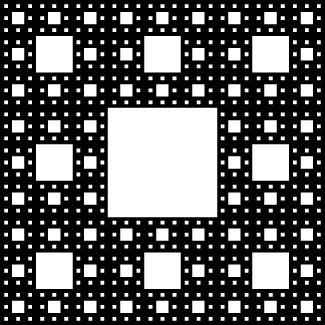
\includegraphics[width=0.3\textwidth]{figs/sierp.jpg}
\vfill

\noindent \hrule
\bigskip
\centerline{\footnotesize \textsc{blank space}}
\vspace{3.0in}
\end{document}